%% $Id$

%% Copyright (c)  1998-2010
%% by  RWTH-Aachen, Germany
%% Some rights reserved.

%% This work is licensed under the Creative Commons Attribution-Share
%% Alike 3.0 License. To view a copy of this license, visit
%% http://creativecommons.org/licenses/by-sa/3.0/ or send a letter to
%% Creative Commons, 171 Second Street, Suite 300, San Francisco,
%% California, 94105, USA.

\section{Coding Styles}
\label{coding_styles}

\subsection{Physical project structure}
Each library which is part of the ViSTA project contains a set of files that should be grouped to \emph{sourcefiles} and \emph{build files}.
For applications (E.g.\ the ViSTA demos), there may be additional \emph{resources} and \emph{configuration} files.

We emphasize the physical separation of these types of files in order to avoid file cluttering that might confuse novice users or developers.
Figure~\ref{fig:ProjectPhysicalLayout} gives an example of a directory tree for an application project.
\begin{figure}[h]
\begin{verbatim}
<project-dir>/
  build/
    built/ [temporary storage, created during compilation]
    msvc9/
    Un*x Makefiles
  configfiles/
    *.ini
  resources/
  src/
\end{verbatim}
\caption{\label{fig:ProjectPhysicalLayout}The physical layout of a project.}
\end{figure}

The following sections will give a brief layout of the depicted folder's content.

\subsubsection{The \code{build} directory}
The \code{build} directory contains all files which are needed for the project to build.
In case a special build directory needs local files to be created during a compilation run, use a separate folder.
For Win32 Microsoft Visual C++ environments, e.g., we differentiate between \code{msvc8} and \code{msvc9} folders at the moment, which contain workspaces, solutions and projects for the respective version of Microsoft compilers.
For Un*x environments, the folder contains the \code{Makefiles} that are needed for the project to build.
The \code{build} directory should also contain a folder that holds all temporarily created data during a compiler run, e.g., object files. 
This folder is typically named \code{built}.
All build environments should create a subfolder below \code{built} and put temporary data which is special to a certain platform and architecture in there.
The idea is to have a single directory which needs to be cleaned in order to remove intermediate files and make a project \emph{distclean}, e.g., before you try to copy it over a slow network share.
Please note that we are currently developing a new \code{cmake}-based build system.
Instructions on how to use it can soon be found in the \code{Documentation} directory going with the ViSTA sourcetree.

\subsubsection{The \code{configfiles} directory}
This directory should hold all initialization files that are needed to run the application or associated tools.
Note that this folder can be used to store auxiliary files, such as data or timing files that may be read by your application.
However, it is possible that many files are needed for a proper configuration of your application, so this folder helps to avoid file cluttering in the main directory.
The \code{vista.ini} is a popular example to store in this directory.

\subsubsection{The \code{resources} directory}
The \code{resources} folder is used to store additional resources that can't really be classified.
As an example, think of bitmap graphics or model files that are not directly needed in the application but are used as sources for application used resources.
It is most useful to collect resource files during the development, as they allow to rebuild some structures in case they are lost.
In addition to this, this folder can hold auxiliary files such as code templates.
It can be used to store some files needed for documentation, e.g., Doxygen configuration files.
It should, however, not be used to store documentation files themselves.

\subsubsection{The \code{src} directory}
This directory contains source and header files, and may even contain some other source file subfolders.
All source files related to the library or application should be contained within this folder.


\subsection{File types and nomenclature}
Each programm is made out of several modules.
We define the atoms to be \emph{classes} that are defined in distinct \emph{files}.
Basically, any file that contains compilable code is called \emph{sourcefile}.
We differentiate between \emph{interface} and \emph{module} files.
The first one is to be used by clients and in C++ usually identified by the \code{.h} suffix,  while the latter one defines the implementation (or module code) and is identified by the \code{.cpp} suffix.

\subsection{File layout and compile time issues}

Any textline in any sourcefile should not exceed 80 characters in width (with 4-spaces-width tabstops).
The reason for this is that it is easier to read inside a window, and in order to print it properly.
All files \emph{must} end with a single endline, as some compilers complain or bail out if it is missing.

All sourefiles in the repository must care for a proper endline encoding.
That means that when checking in on Un*x platforms, all code has Un*x endline encoding, whereas code checked in on Win32 has Windows/DOS endline encoding.
Please try to avoid code copied between Un*x and Windows platforms in any case, or convert the endline encodings properly before checking in to the repository.


For the indentation of source lines, TAB-stops should be used.
The indention-behaviour should be configurable in any decent text-editor or programming environment.
If you encounter a file which is improperly formatted (in any respect), please reformat it according to this styleguide.
Many advanced editors, like e.g. Microsoft Visual C++ or Emacs, offer functions and macros to do this automatically for whole files/regions.

\subsubsection{Platform and system dependant preprocessor directives}
Currently, at some point, an operating system specific compilation is required.
In \code{ViSTA}, we define operating system types as given in Table~\ref{tab:OSTYPES}.
\begin{table}
	\centering
		\begin{tabular}{l p{7cm}}
		LINUX & All types of Linux derivates \\
		SUNOS & Sun Solaris \\
		HPUX & Hewlett Packard OS \\
		WIN32 & Windows \\
		IRIX & SGI's Irix OS \\	
		DARWIN & Apple's Mac OS X \\	
		\end{tabular}
		\caption{\label{tab:OSTYPES}Preprocessor directives for system and system dependent options.}
\end{table}
A define as given in the table is defined during a compilation run and can be queried, using, e.g., the \code{\#if de\-fin\-ed(LINUX)} directive.
Note that, right now, we do not really differentiate between different processor architectures, e.g., LINUX on a 64bit machine.
Additionally, sometimes the platform compilation really means a compilation for different compilers and not the machine, e.g., some code works for the \code{gcc}, but not for the \code{CC}, although the \code{gcc} and the \code{CC} can both be used on SUNOS.

\subsubsection{Module reference style}
Sourcefiles include other interface, e.g., header files.
When doing this the following rules apply.
Any inclusion of an interface file clearly identifies a dependency, as at least at compile time the other files have to be present.
\begin{itemize}
\item Please remove references to files that you do not really need inside of a header file.
\item Be aware of modularity: include files that reside in the same module must be referenced using the local inclusion directive 

\code{\#include "localcompanion.h"}.
\item Modules that reside in submodules must be included using the local inclusion directive 

\code{\#include "module/localmodule.h"}.
\item Modules from other modules, e.g., system or other library modules, shoud be resolved using the global inclusion directive 

\code{\#include <VistaKernel/VistaSystem.h>}.
\item Try to avoid relative inclusion, although feeling the temptation to do so. \textbf{Do not use} the following.

\code{\#include "../uppermodule.h"}.

If you feel that this is appropriate, think about your module layout in general, something might be wrong.
\end{itemize}

\subsubsection{Interfacefile (\code{.h}) layout}
%% TODO reference template section here
All header files must contain the proper header for the license in use (LGPLv3 at the moment).
After the copyright message, each header must contain the SVN id tag like depicted in the following.

// \code{\$Id\$}

%\begin{verbatim}
%// $Id$
%\end{verbatim}
Remember that SVN does not do keyword substitution by default (like CVS) but that it has to be explicitly enabled for new files that are added to the repository. This is done by setting the SVN property \code{svn:keywords Id} with your favourite SVN client. Also remeber to set the property \code{svn:eol-style native} for code files.
A header file must define so called \emph{include guards}.
Include guards in C/C++ are preprocessor defines that are defined when a header file is encountered first.
This technique avoids double inclusion of header files and some serious compiler trouble.
Include guards should reflect the file name as close as possible.
For example, the header file \code{MyClass.h} defines the include guard as follows.
\begin{verbatim}
#ifndef _MYCLASS_H
#define _MYCLASS_H

... <code here> ...

#endif // _MYCLASS_H<endl>
<endl>
\end{verbatim}
The idea behind this technique is that a sourcefile resembles the class that is contained in it.
A class is a type, and a type must be unique during one compile time run.
As a consequence, using the class name as an include guard assures uniqueness in most cases.
Please use only \textit{single underscores} for your include guard defines, as defines beginning with a double underscore are reserved by most compilers.

%\subsubsection{Module reference constraints}

A sourcefile should only include other source header files that are absolutely needed in order to compile the source file.
In detail, this means that other headers should only be included for reasons of inheritance and aggregation of other types.
\begin{itemize}
\item Please overcome the temptation to include "files you usually need when you need this class".
\item Use opaque forward declarations and pointer or reference constructions when aggregating other types.
\item Please try to group the forward declarations with respect to their origin.
\item You must remove types from the list of forward declarations if you do not really need them anymore.
\item Avoid the inclusion of "utility" headers, e.g., \code{stdio.h, math.h} or others the like.
\item Every header file \textbf{must} be finished with a single endline.
Some compilers bail out if a file is not finished by an endline, most utter a warning.
\end{itemize}

\minisec{Shared Library Exports}

On the Windows platform, classes and types that should be exported into a shared library (DLL) need special handling.
For the \code{ViSTA} core libraries there are macros defined to account for this. 
Typically, you find them for each module in a top-level header file named \code{Vista*Config.h}.
You have to place these macros between the \code{class} keyword and the symbols that should be available in the DLL you are going to create.
%% Another special case arises when dealing with template instances and shared libraries.
%% All templates that your class will instantiate have to be exported into the DLL. 
%% Again, there are macros defined to handle import/export of template instantiations when building/using the \code{ViSTA} core libraries. 
If you are building the library itself, the define \code{VISTA[LIB]\_EXPORTS} has to be set (e.g. \code{VISTAMATH\_EXPORTS} for VistaMath). 
However, if you want to build a static version of the library, you may set the define \code{VISTA[LIB]\_STATIC} to deactivate exporting of symbols. Note that static libraries are not officially supported!
For applications building \textit{against} the \code{ViSTA} base libraries, no special defines need to be set.

Import/export handling macros: \code{VISTA[LIB]API} \\
Preprocessor macros to switch off library imports in your build: \code{VISTA[LIB]STATIC}

Where \code{[LIB]} depicts the appropriate library name \code{ASPECTS}, \code{INTERPROCCOMM}, \code{TOOLS}, \code{MATH}, \code{DEVICEDRIVERS}, \code{DFN} or \code{KERNEL}.

The following code gives an example for a class in the VistaKernel library:
%\lstset{language=C++}
%\lstset{basicstyle=\small}
%\begin{lstlisting}
\begin{verbatim}
#include <VistaKernel/VistaKernelConfig.h>

class VISTAKERNELAPI VistaMyFancyClass
{
  public:
    // nested classes need to be exported explicitly
    class VISTAKERNELAPI CNestedClass
    {...}

    // (see below for explicit export)
    vector<COtherClass> m_vecObjects;
	  
  private:
    // private declarations usually are not exported...
    class CPrivateUtiliyClass
    {...}
};
\end{verbatim}

%\end{lstlisting}


\subsubsection{Modulefile (\code{.cpp,.c}) layout}
Module files are a bit simpler in layout.
Each module file must also contain a proper license header as shown in the code template.
After that, the module file should be split into the following four sections:
\begin{enumerate}
\item Include section
\item Local classes, variables and functions section
\item Constructor/Destructor section
\item Implementation section
\end{enumerate}
%% TODO reference code template section 

\minisec{Include section}
A module file must contain a SVN Id tag, just as the header file.
The first thing to appear in a module file is the \emph{include section}.
The following order is recommended, but may vary if needed.
\begin{enumerate}
\item Self interface inclusion. 
That means the interface for the classes that are implemented in the module file should be included first.
\item Local modules. 
Include all modules that reside in the same module or in submodules.
\item Global or non-local modules.
Include modules from upper or global modules. 
Try to group the modules according to their source.
If in doubt, try to put in a comment, why you need this inclusion.
\item System wide includes.
Reference system includes last.
\end{enumerate}
Note that the above order is not strict, but should be respected.
Sometimes it helps to navigate and to see compile dependencies at a short glance.

\minisec{Local/Static section}
Local classes, functions and variables should be declared using anonymous namespaces to hide them from other modules and to not pollute the global namespace.
Class variables go here (into this section, but not into an anonymous namespace), too.

\begin{verbatim}
// <wrong code>
// private module variable
const float mypi = 3.14f;
// </wrong code>

// <bad code>
// private module variable
static const float mypi = 3.14f;
// </bad code>

// <better code>
namespace
{
// private module variable
static const float mypi = 3.14f;
};

// class variables go here, too - note that they of course
// mustn't go into the anonymous namespace!
int CMyClass::m_SMyStaticVar = 0;

// </better code>
\end{verbatim}


\minisec{Constructor/Destructor section}
The next thing to define is the \emph{constructor/destructor} section that defines \emph{all} constructors and destructors for all classes as defined locally or in the interface file.
Try to group all constructors and destructors in a sequence for a single class.
Try to mark the end of a constructor/destructor sequence for a class with appropriate comments.
For example, see the following code, that can be found in \code{A.h}.
\begin{verbatim}
class A
{
 public:
  A();
  virtual ~A();
  
  class B
  {
   public:
    B();
    virtual ~B();
  };
}; 

class C
{
public:
	C();
	virtual ~C();
};
\end{verbatim}
This declaration leads to the following sequence in the module file:
\begin{verbatim}
#include "A.h"

A::A() {}
A::~A() {}
// ##########################
A::B::B() {}
A::B::~B() {}
// ##########################
C::C() {}
C::~C() {}
// ##########################

<begin implementation section here>
\end{verbatim}

\minisec{Implementation section}
For the implementation section, there are no rules about its layout.
You can try to group certain methods of the classes' interfaces and you can try to mark the layout of the functions with appropriate comments.
As most tools allow GUI browsing in the source code and bookmarks, it is not really enforced to keep with a specific order.
Please try to avoid local declaration and definitions of statics (variables of functions) in the implementation section.
When implementing different classes, you should, however, group the implementation of the classes in the implementation section.

Just as in the interface file, end all module files with a properly encoded endline.


\subsection{Module Syntax}

\subsubsection{Hungarian notation table}\label{sec:HungarianNotation}
The Hungarian notation is useful as it allows to deduce a variable type from its name.
This is realized by defining a symbolic mapping for prefixes of variable names to an intended type.
We know that there are several reasons against using Hungarian notation in a typed language like C++.
However, we employ a "lazy" symbolic typing, as we assume that specific prefixes can be used for classes of specific types.
First of all, \textbf{design hints} are important for developers to classify types and members at short glance.


\begin{tabular}{|l|l|p{10cm}|}
\multicolumn{3}{c}{\textbf{Design hints}}\\\hline
\textbf{Prefix} & \textbf{Target} & \textbf{Purpose} \\\hline

none   & Classes & Applicable as prefix to classes that have an implementation,
              e.g., members, methods and a protocol. You should not use
              this prefix for classes that resemble an interface.\\\hline
I   & Interfaces, Class & Defines an interface class. Usually interfaces
                        can easily be identified as classes that contain
                        a large number of pure virtual methods and have
                        no or a small number of members and not a real
                        protocol.\\\hline
m\_ & Member prefix & All class and struct members \emph{must} be prefixed
                      with the m\_. This really is important as it helps
                      to identify member variables when searching code
                      from other developers.\\\hline
\end{tabular}

Primitve types in the C/C++ language. 
We do not give prefixes for all possible types, but for the mostly used types.

\begin{tabular}{|l|l|p{10cm}|}
\multicolumn{3}{c}{\textbf{Primitive types}}\\\hline
\textbf{Prefix} & \textbf{Target} & \textbf{Purpose} \\\hline
a   & C/C++ array types & Use for signed or unsigned arrays or other types.\\\hline
b   & bool               & C++ boolean types\\\hline
c   & chars & Basic char types\\\hline
d   & double & Applicable to double primitive types.\\\hline
f   & floats & Applicable to float types.\\\hline
i   & integer & Applicable to integer types. \\\hline
n   & basic number types & We consider the n prefix for all types of numbers.
                          You can use n as prefix for doubles, floats and
                          integers.\\\hline
o   & referenced instances & Applicable to references to other objects
                           and aggregates.\\\hline
p   & pointer types & Apply this prefix to pointer types.\\\hline
\end{tabular}

Types are nice, but usually they are associated with attributes, e.g., static or singed/unsigned qualifiers.

\begin{tabular}{|l|l|p{10cm}|}
\multicolumn{3}{c}{\textbf{type attributes}}\\\hline
\textbf{Prefix} & \textbf{Target} & \textbf{Purpose} \\\hline
e   & enums & Enums are integers, basically, but try to identify them
              by using the enum prefix.\\\hline
S   & static variables & You can use this for static variables and infix for
                       static members or module variables.\\\hline
u   & unsigned type & Optional, but can be used for unsigned types.\\\hline
\end{tabular}

As STL containers are used throughout the interfaces, we define prefixes for the most commonly used STL types.

\begin{tabular}{|l|l|p{10cm}|}
\multicolumn{3}{c}{\textbf{STL types}}\\\hline
\textbf{Prefix} & \textbf{Target} & \textbf{Purpose} \\\hline
li  & lists & STL list types\\\hline
map  & maps  & STL maps\\\hline
str   & string types & STL strings \\\hline
vec  & vector & Vectors from the STL\\\hline
qu   & queue & Queues and dequeues from the STL\\\hline
\end{tabular}


For ViSTA applications, the usage of VistaMath objects is common.
The following table defines naming conventions for objects of the VistaMath library.

\begin{tabular}{|l|l|p{10cm}|}
\multicolumn{3}{c}{\textbf{Common types in ViSTA}}\\\hline
\textbf{Prefix} & \textbf{Target} & \textbf{Purpose} \\\hline
v3  & Vectors &  VistaVector3D\\\hline
q  & Quaternions & VistaQuaternion \\\hline
mat   & Matrices & VistaTransformMatrix\\\hline
\end{tabular}


\subsubsection{Interfaces}\label{sec:ClassCoding}
Interfaces are the primary source of information for developers.
So a consequent layout is mandatory in order to help other developers in their task to understand the functionality of the interface.

\minisec{Choosing types}
\begin{itemize}
\item Try to prefer classes to structs as modelling primitives.
Always provide constructors and destructors for classes.
Initialize all members of the class to a valid state in its constructor.
\item Identify interfaces (specification) and concrete classes (implementation).
Try to model as much as interface as possible.
Use the "I" prefix with care.
\item Embed "local" classes in the parent class in which they are used.
For example, a helper class that does not make sense outside of the scope of a certain class should be modeled as a public or private class inside of the interface or inside of the module file.
\begin{verbatim}
class C
{
 public:
  class myPublicHelper 
  {
  public:
   myPublicHelper();
   virtual ~myPublicHelper();
  };
  
private:
  class myPrivateHelper
  {
	  // consider moving this private
	  // class inside the module (C.cpp) file,
	  // as it pollutes the "interface"
	  // that is accessible for clients of this
	  // interface
   public:
   myPrivateHelper();
   virtual ~myPrivateHelper();
  };
};
\end{verbatim}

\item Avoid the use of \code{\#define} constructions at any cost.
If you need symbolic number mappings, use embedded \code{enum} constructions.
\begin{verbatim}
<badcode>
#define MY_FIRST_SYM 1
#define MY_NEXT_SYM 2

class C
{
public:
  // pub sym is expected to by one of
  // the above
	C(int pubSym)
	virtual ~C()
};
</badcode>

<bettercode>
class C
{
 public:
 enum
 {
   MY_FIRST_SYM = 1,
   MY_NEXT_SYM
 };
 
 C(int pubSym);
 virtual ~C();
};
</bettercode>

<evenbettercode>
class C
{
 public:
 enum eSyms
 {
   MY_FIRST_SYM = 1,
   MY_NEXT_SYM
 };
 
 C(eSyms pubSym);
 virtual ~C();
};
</evenbettercode>
\end{verbatim}
\end{itemize}

\minisec{Naming rules}
Classes and structures must be named in order to identify their functionality.
Try to be as verbose as possible.
\begin{enumerate}
\item Identify interface functionality with a property postfix, e.g., \code{IVistaNameable} uses the postfix "able" to state the subclasses fulfill a specific functionality.
\item Identify high level functionality that is congruent to other classes, e.g., \code{Vista\-Trackball\-Behavior} states that the class realizes a concept of a behavior, although there is no abstract interface or explicit concept "behavior" anywhere in \code{ViSTA}.
The same accounts to all \code{Manager} classes in \code{ViSTA}, as there is no base class in \code{ViSTA} for "management" classes.
Another example can be seen in \emph{implementation} classes, that are postfixed with \code{Imp}.
\item Use project specific prefixes after the type prefix.
E.g., new \code{ViSTA} core classes must be prefixed with \code{Vista}, for example \code{Vista\-My\-New\-Core\-Class}.
If you are writing potential \code{ViSTA} classes as part of a project, choose a project specific prefix and use it!
When, for example due to refactoring, classes are moved between libraries or projects, renaming to the new project prefix helps to move them first, migrate the old code to the new layout and finally removing old classes.
Alternatively, especially for new libraries or projects, we recommend the use of \code{namespace}s to clearly specify where a class belongs to but keep class names short. Moving to other modules is easier also, as in most user code you just need to change a single \code{using namespace} line.
\end{enumerate}


\minisec{Members and methods}

\minisec{Members and other variable names}
Variable names play an important role in understanding code from strangers.
Differentiate between the following member or variable types.
\begin{itemize}
\item Members. 
Members are variables within class scope. 
Always prefix members of classes or structs with \code{m\_} to point out that they belong to the current instance.
\begin{verbatim}
<badstyle>
struct s 
{
	int a;
	int b;
};
</badstyle>

<goodstyle>
struct s
{
	int m_a;
	int m_b;
};
</goodstyle>
\end{verbatim}
\item Module variables.
Modules can contain private variables that are not important outside of the module.
First of all, module variables should always be qualified with the \code{static} initializer to prevent external linkage.
Second, it is helpful to prefix static variables with an uppercase \code{S}.
\begin{verbatim}
<badstyle>
#include <....
...
int modulevar = 5;
...
</badstyle>

<goodstyle>
#include <....
...
static const int Smodulevar = 5;
...
</goodstyle>
\end{verbatim}
\end{itemize}
In general, respect the hungarian notation as defined in section~\ref{sec:HungarianNotation}.
Prefixing member variables with \code{m\_} is mandatory while selecting a proper type-prefix should be based on common sense.

\minisec{Method signature}
The term "method" stands for all functions, operators and constructors and destructors or a class.
However, some constraints apply to theses different types of methods.
For the general case, we define the following rules.
\begin{itemize}
\item All methods start with an \emph{uppercase letter}. 
In addition to that, we avoid the use of underscores in the function name.
Inlined terms are separated using uppercase letters again (aka "CamelCase").
\begin{verbatim}
class C
{
 public:
 C() {}
 virtual ~C() {}
 
 // illegal
 int getNumber() const;
 int _getNumber() const;
 int _get_number() const;
 int Get_number() const;
 int Get_Number() const;
 
 // legal
 int GetNumber() const;
};
\end{verbatim}
\item Parameter types differentiate between \emph{in-} and \emph{out-}parameters.
Use the \code{const} qualifier to identify \emph{in-} parameters, that is parameters that are not changed as a side effect inside the method.
\begin{verbatim}
class C
{
 public:
 C() {}
 virtual ~C() {}
 
 
 // nArgA and nArgB are processed,
 // the result is stored in nResult
 bool Calculate(int nArgA, 
                int nArgB, 
                int &nResult); 

 // alternativly: explicitly state that nArgA and nArgB
 // are in-parameters by using the 'const'
 bool Calculate(const int &nArgA, 
                const int &nArgB, 
                int &nResult);
};
\end{verbatim}
In the example above, the method \code{C::Calculate()} receives \code{argA} and \code{argB} as in-parameters that are not changed inside of the method in any way, whereas nResult is an outgoing parameter, indicated by the non-const reference type.
\item Use const reference types when arguments are in-paramters and mandatory.
Using const references avoids the in and out copying of temporaries and temporaries may be passed when calling the methods (not all compilers are yet smart enough to skip unnecessary copies).
\begin{verbatim}
class C
{
 public:
 C() {}
 virtual ~C() {}
 
 // wrong or at least bad
 bool SetNameForNameable(std::string sName);
 
 // better and the desired way to do!!
 bool SetNameForNameable(const std::string &sName);
};
\end{verbatim}
\item Use pointer types for optional arguments.
Pointers, in contrast to references, can be NULL.
This indicates that NULL can be passed as an argument.
Specify in your method documentation if this is invalid.
\begin{verbatim}
class C
{
 public: 
 // pointer types indicate optional arguments
 void Associate(int nToken, C *other);
 
 // note that the above needs additional documentation!
};
\end{verbatim}
\item Syntax: please respect the 80 character constraint in the method signature syntax.
Enter endlines after each argument, or at places that look appropriate.
\begin{verbatim}
class C
{
 public: 
 // put in endlines in order to avoid 
 // lines longer than 80 chars.
 // try to reference the first argument
 // after the method name
 void Associate(int nToken, 
                const std::vector<float> &vecFloats,
                float fOther
                C *other);
                
 // we dislike the following notation, 
 // do not disrupt return type and method name
 void
 Associate
  (int nToken,
  const std::vector<float> &vecFloats,
  float fOther, 
  C *other);
};
\end{verbatim}
This rule applies to interface and to module files respectively.
\item We do \emph{not} apply Kerningham-Ritchie style C bracketing for methods, switch/case statements or loops.
Put braces to blocks in distinct lines, with, at most, only comments accompanying it.
\begin{verbatim}
<badstyle>
// loops
for(int n=0; n < 5; ++n) {
 foo();
}

// methods
void C::foo() {
}

// switch/case
switch(nType) {
 case 1: {
 	break;
 }
 default: {
  break;
 }
}
</badstyle>

<goodstyle>
// loops
for(int n = 0; n < 5; ++n) 
{
 foo();
}

// methods
void C::foo() 
{
}

// switch/case
switch(nType) 
{
 case 1: 
 {
 	break;
 }
 default: 
 {
  break;
 }
}
\end{verbatim}
\item Use block braces in switch/case blocks.
\begin{verbatim}
<badstyle>
switch(nType)
{
 case 1:
 	break;
 default:
  break;
}
</badstyle>

<goodstyle>
switch(nType)
{
 case 1:
 {
  break;
 }
 default:
 {
  break;
 }
}
</goodstyle>
\end{verbatim}
The above does not look too nice, but is necessary to correctly scope your local variables, especially when doing nested \code{switch/case} blocks.
\item Do not brace non-complex return values.
\begin{verbatim}
<badstyle>
bool C::GetIsEnabled() const
{
 return (m_bIsEnabled);
}
</badstyle>

// it is ok to brace 'complex' returns
<goodstyle>
bool C::GetIsEnabled() const
{
 return (GetIsNotDead() && m_bIsEnabled);
}

bool C::GetIsEnabled() const
{
 return m_bIsEnabled;
}
</goodstyle>
\end{verbatim}
\end{itemize}

\minisec{Method implementation}
First of all, try to avoid defensive programming.
That means, do not try to detect a proper state within every single method at the beginning.
In general, it is better to give users a clear outline of the protocol of the class, than to check every argument twice, thrice or thousands of times.
However, during development, it is very ok to check for valid states.
Please check the validity of the instance state only at the beginning and abort processing when a desired state is not present.
\begin{verbatim}
class C
{
 <...>
 /**
  * Precondition: GetC() != NULL
  * Postcondition: if this method returns true,
                   we really did da C
  */
 bool DoDaC();
 
 C *GetC() const { return m_pC; }
private:
 C *m_pC;
};

<bad style>
bool C::DoDaC()
{
	if(m_pC)
	{
		<thousands of lines of code>
		...
	}
	else
		return false;
	
}
</badstyle>

<good style>
bool C::DoDaC()
{
	if(!m_pC)
		return false;
	
	// assume that m_pC != NULL for the
	// rest of this method
	
	<thousands of lines of code>	
}
</good style>

<even better>
bool C::DoDaC()
{
	// user was told to check for m_pC
	// *before* calling DoDaC()
	
	<thousands of lines of code>
	...
	
	return (weDidDaC == true);
}
</even better>
\end{verbatim}

\minisec{Constructors/Destructors}
\emph{Always} provide constructors and destructors for your class.
For constructors, think about the following.
\begin{itemize}
\item Provide \emph{public default constructors} which initialize \textbf{all} variable members with proper values that enable instance functionality.
Prefer constructor base type construction to explicit construction in the body of the constructor.
\begin{verbatim}
class C
{
 public:
 C()
 // prefer to initialize base members
 // in construction list
 : m_nCnt(0),
   m_bValue(false),
   m_veInts()
 {
  // no need to do the following:
  m_veInts.clear();
  // it is done in std::vector<int> constructor
  // anyways, so do not do it again.
 }
 
 virtual ~C();
 
 private:
 int m_nCnt;
 bool m_bValue;
 
 std::vector<int> m_veInts;
};
\end{verbatim}
\item Provide \emph{protected constructors} for classes that you consider to be derived and instantiated, rather that instantiated directly.
For classes like these, provide a \emph{protected copy constructor} to prevent copying by others that the specialized classes.
\begin{verbatim}
class C
{
public:
 // we assume that C has to be derived,
 // so we define the destructor to be virtual!
 virtual ~C();
 
protected:
  C(); // default constructor
  C(const C&); // ANSI-C copy constructor
  C &operator=(const C &other); // protected assignment
};
\end{verbatim}
\item Provide \emph{special public constructors} if you can't initialize an instance properly with a default constructor.
\begin{verbatim}
class C
{
public:
  // in this example, we can not determine
  // our index in a default construction
  // so we pass it explicitely
 C(int nIdx)
 : m_nMyIdx(nIdx) {}
 
 virtual ~C() {}
private:
  int m_nMyIdx;
};
\end{verbatim}
\item Think about deep or shallow copy properties of your class!
Whenever you aggregate pointer types as members, this can be crucial.
When deep copy semantics have to be applied, be sure to provide \emph{copy constructors} \textbf{and} \emph{assignment operators}.
For shallow copy semantics, you may be ok with the default copy constructor or the assignment operator.
\begin{verbatim}
class DeepCopyC
{
public:
 DeepCopyC()
 : m_pveMyVec(new std::vector<float>) {}
 
 DeepCopyC(const DeepCopyC &other)
 {
   m_pveMyVec = new std::vector<float>;
   (*m_pveMyVec) = (*other.m_pMyVec);
 }
 
 virtual ~DeepCopyC()
 {
  // it is ours, so we can delete it
  // safely
 	delete m_pveMyVec;
 }
 
 DeepCopyC &operator=(const DeepCopyC &other)
 {
  // check if other is me ;)
 	if(this != &other)
 	{
   m_pveMyVec = new std::vector<float>;
   (*m_pveMyVec) = (*other.m_pMyVec);
  }
  return *this;		
 }
private:
	std::vector<float> *m_pveMyVec;
};
\end{verbatim}
\end{itemize}
For destructors, think about the following.
\begin{itemize}
\item Try to make destructors with \emph{public access} attribute in general.
\item All classes that can be potentially derived \emph{must} (I repeat: \emph{must}) have a virtual destructor!
Please provide this virtual destructor \emph{as the \textbf{first public} method} in the interface.
\item For all classes which are not considered to be derived at all, some developers declare the destructor as non-virtual to indicate for other developers that you should not derive from that class.
Since this technique is very error-prone, we recommend to declare \emph{all} your destructors as virtual and rather describe why the class should not be inherited from in the interface documentation.

\begin{verbatim}
class C
{
public:
	C();
	
	// always declare your destructors virtual
	virtual ~C();
};
\end{verbatim}
\item Sometimes, destructors can \emph{invalidate} members, which will raise a definite error, for example when deleted instances are use somewhere in the code.
Feel free to invalidate pointers, but avoid to invalidate aggregates.
\begin{verbatim}
class C
{
 virtual ~C()
 {
  // invalidate pointer
  // set it to 0 so that dereferencing afterwards
  // certainly produces an error
  m_pOtherC = (C*)0x0; 
  // btw: we assume that some other instance
  // cares about the memory that is pointed
  // at with m_pOtherC
  
  // BAD, DO NOT DO THE FOLLOWING, AS IT IS
  // OF NO DEEPER MEANING BESIDES WASTING
  // CPU CYCLES:
  m_veOtherCs.clear();
 }
private:
  C *m_pOtherC;
  std::vector<C*> m_veOtherCs;
};

\end{verbatim}
\end{itemize}

\minisec{Operators}
We do not emphasize the overloading of operators in classes.
The only good place to use overloaded operators is in mathematical classes, as in these environments constructions get more readable.
When defining operators, be sure to respect the original semantics of operators and do not try to implement something that is totally different and might confuse other developers.

\minisec{Getter methods}
Getter methods return values of members or a deduction from private properties.
In any case, getter methods \emph{must not change the state} of an instance and thus all carry the \code{const} qualifier.
\begin{verbatim}
class C
{
 public:
 C() : m_nA(0), m_nB(1) {}
 
 virtual ~C() {}
 
 int GetA() const  { return m_nA; }
 int GetB() const { return m_nB; }
 int GetSumOfAAndB() const { return m_nA + m_nB; }
 
 private:
 int m_nA, m_nB;
}; 
\end{verbatim}
Please make your interface as \emph{const-correct} as possible!
If your method does more than a simple "get", then do not call it "getter" and reflect what it does in the method name.

\minisec{Setter methods}
Setter methods might indicate the success of setting a value by returning a boolean value.
This is not mandatory, but might be useful to the programmer calling the set method.
The documentation of the setter method should indicate how the object's state is changed after the setter.


\minisec{Members}
Member variables must respect the hungarian notation, as given in section \ref{sec:HungarianNotation}.
Try to be very verbose when designing the member name. 
If you change the type of the member, adapt to the new type in the hungarian notation.
"Search \& Replace" is a handy feature of your most favourite editor here.


\minisec{Inheritance}
As a rule of thumb, use inheritance to reflect only \emph{is-a} relations between classes.
Whenever you feel the need to use inheritance for code re-use, please think again if the desired code re-use can not be modelled using the \emph{has-a} relationship.
Avoid multiple inheritance if you can.
There can be exceptions, but please consider these carefully.
There is usually no sense in private inheritance (this is simple code re-use that is better embodied as a \emph{has-a} relationship), and there seldomly is sense in protected inheritance, so do only consider public inheritance.

However, if you design your class to be inherited, please try to clear your attitude to other developers.
Use protected methods to indicate where other developers have a chance to intercept the classes' protocol.
Do not use protected members, but use private members and protected getters and setters in order to remain control of the state of the instance.
Always provide virtual destructors for classes that can be inherited from.

\minisec{Memory management}
In C++, you have to deal with memory management without the luxury of a garbage collector.
Please be aware of that.
In general, be aware of \emph{responsibilities} for the lifetime of instances.
That means that you should point out in interface and documentation, which instance is responsible for the memory management of associated instances.
\begin{verbatim}
class C
{
 /**
  * @param a a pointer to an A, a is deleted, 
             when this C is deleted, too
  */
 C( A *a)
 : m_pA(a) {}
 
 virtual ~C()
 {
 	delete m_pA;
 }
 
 /**
  * @return returns a pointer to the internal
            A, do not delete that pointer,
            as it belongs to this C
  */
 A *GetA() const { return m_pA; }
 
 /**
  * @param a a pointer to another A,
             the pointer is simply copied and this C thinks
             that it will own a. The old a is forgotten
             and not deleted.
  */
 void SetA(A*a) { m_pA = a };
 private:
 A *m_pA;
};
\end{verbatim}

\minisec{Data hiding and encapsulation}
\begin{itemize}
\item \emph{Inheritance}: you \emph{must not} use protected inheritance and avoid private inheritance \emph{at all costs}.
Use public inheritance in almost all cases you can think of.
\item \emph{Member access policies}: Instance variables should have \emph{private} access and only be available by public methods.
This should usually be true even for derived classes, do not use protected variables.
There are exceptions: when desinging "data carriers", classes without protocol, you can decide to use all members in the public signature of the class.
For example, the follwing class does only carry some values, but there is no direct dependency between these values, and there is no need for an interface.
\begin{verbatim}
class C
{
	public:
	C()
	: m_unId(0),
	  m_nDeltaT(1.0f) { }
	  
	virtual ~C() {}
	
	unsigned int m_unId;
	float        m_nDeltaT;
};
\end{verbatim}
As a consequence, there is no need for privacy and using getter methods is overhead that can be avoided.
Classes like the above are usually used for the construction of others or when some data is transported across module boundaries.
\end{itemize}

\subsubsection{Sourcefiles}
Sourcefiles embody the \emph{physical modules}, especially when working with revision control systems, e.g., CVS or subversion.
In principle, a single sourcefile should contain a single class, where the class has a very similiar name to the sourcefile. 
For example, the \emph{interface} to the class \code{CMyImportantObject} should reside in a sourcefile named \code{MyImportantObject.h}.
The \emph{code} for that class should reside in a sourcefile named \code{MyImportantObject.cpp}.
The sourcefile name should not reflect the qualifier of the class, that means the prefix, "C" in this example, should not be part of the filename.
Exceptions may be made when designing interfaces that use the prefix "I", in order to gather \emph{interface-classes} physically in the filesystem view.

These naming rules are \emph{mandatory}, as it eases the navigation inside the source code, especially in larger projects.
If a project developer decides to rename a class, for whatever reason, the source file must be renamed properly.
Note that this can mean to remove and add a module from the version control system.

Sourcefiles should usually not contain more than one class.
The exceptions to this rule are \emph{local classes}, that is classes that are bound to the sourcefile's class as substructures.
Another exception may be made when using template code to offer some implementation alternatives to a single class.
Figure~\ref{fig:sourcefiles} shows the defined rules in a picture.
\begin{figure}
\begin{center}
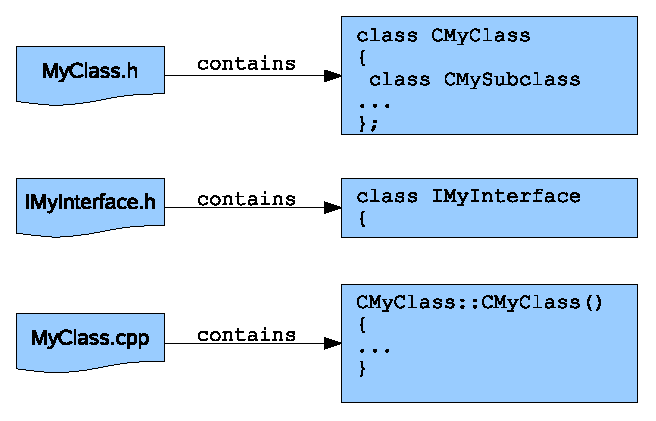
\includegraphics[width=10cm]{sourcefiles}
\end{center}
\caption{\label{fig:sourcefiles}
        Sourcefiles and allowed relationships to the classes and interfaces they can contain.}
\end{figure}


\subsection{Source code documentation}
For all documentation either in the interface files or in the module files, we apply \emph{Doxygen} comments, in the \emph{Javadoc} style.
For interface syntax, see section \ref{sec:ClassCoding}.
All documentation should be written in english, of course.

\subsubsection{Interface file documentation}\label{sec:InterfaceDocumentation}
The interface is the primary source of interest to programmers that like to figure out what an instance of a certain class is all about and how the protocol is defined to use it.
The documentation of the interface should consider these aspects very carefully.
The following rules apply to the documentation of interface files.
\begin{itemize}
\item Do \emph{not} bother to document classes that you currently develop or that you have developed recently in the interface file itself. 
The reason for this is that classes that are under development change heavily, but usually comments will not be updated properly.
This misleads other developers once they try to use the interface.
Concentrate on test cases and demonstration programs, in order to point out the interface.
\item Do comment all interfaces once you notice that the interface gets more and more stable.
Focus on the class documentation first, try to depict the protocol of the class in detail.
Especially, do comment the interface once other developers come to you and ask questions about its usage, or if you notice that your class is not properly used by others.
\item Do not comment the obvious, unless there is something not obvious.
\begin{verbatim}
<bad>
 /**
  * Sets the name of this instance.
  * @param sName the name to be set
  */
 void SetName(const std::string &sName);
 
 /**
  * Gets the name of this instance.
  * @return the name of this instance as a string
  */
  std::string GetName() const;
</bad>
\end{verbatim}
This is not very helpful, as the method names and return types document what they are supposed to do.
\item Try to document things that are not obvious, especiall the relations to other classes and instances.
Try to point out the pre- and postconditions if you can and if they are important.
\begin{verbatim}
<good>
 /**
  * Sets the name of this instance and tries
  * to register it with the global object registry.
  * If this fails, e.g., the name is already taken
  * by another instance, this method will
  * throw an exception.
  * Note that the name can only be set once and is
  * then considered immutable. If it is tried to set
  * it again, an exception is thrown.
  * Pre-condition: the name was not set and
                   no instance with that name
                   was registered to the object
                   registry before, e.g, 
                   ObjectRegistry::GetInstance(sName) must
                   return NULL
  * Post-condition: this->GetName() returns sName, which is
                   not the empty string,
                   and ObjectRegistry::GetInstance(sName)
                   returns a pointer to "this" with the
                   name "sName". A subsequent call to
                   SetName() will raise an exception.
  * @param sName the name to be set, must not be 
                 the empty string and should be
                 unique in the namespace of this
                 object's object registry.
  */
 void SetName(const std::string &sName);
</good>
\end{verbatim}
As you can see, sometimes, even methods with simple names do a little more than their name reveals, and this is \emph{not} considered to be good practice.
\item Group methods that are used for a specific aspect of the class/instance.
Especially, group all methods that override virtual methods from superclasses and mark this with a comment.
\begin{verbatim}
class C : public IVistaNameable
{
public:
	  C();
	  virtual ~C();
	  
	  // #############################################
	  // C-class specific interface
	  // #############################################	  
	  bool MyCFoo();
	  
    // #############################################
    // (SPECIALIZED) NAMEABLE INTERFACE
    // #############################################
    virtual string GetNameForNameable() const;
    virtual void   SetNameForNameable(
                             const string &sNewName);
};
\end{verbatim}
\end{itemize}

\subsubsection{Module file documentation}
Module files contain the source code and thus the implementation of a class. They are usually of interest to other developers when they have to enhance the code, to understand a non documented protocol or if they appear to have found an error.
For module file documentation, the following rules apply.
\begin{enumerate}
\item Try to document passages that are difficult to understand, try to avoid too obvious comments that mislead interpretations.
\item Try to point out some pre- and postconditions for methods. 
E.g., be precise when a class does expect a certain protocol, or the outliving of resources (pointers to members that are deallocated by others).
Usually, instances implement a protocol of how to use them.
This protocol has to be pointed out very clear in the documentation, sometimes even in the module file.
\item Whenever you find a method that you implemented yourself, and you do not understand it anymore, \emph{write a comment} once you understand it again!
The chance that other people, who did not write the routine, do not understand your code, is very high here.
\item Please do not feel urged to write comments about methods that \emph{change frequently}, or that are \emph{simple to understand}.
In object-oriented programming, methods should be short and to the point, so they are, as routines themselves, not hard to understand (most of the times).
\end{enumerate}
However, it is good practice to give some navigation hints with commentary to other developers, e.g., marking the beginning of a new class implementation in the implementation section with broad comments, for example with a large number of hashes or asterisks.

\subsubsection{Compiler Warnings}
Someone said: ''Warnings can be ignored''.
Although true to some extent, warnings always give rise to insepct some issue with a code a little deeper.
The general advice is thereby: ViSTA code compiles without warnings.
There is three basic ways of dealing with warnings:
\begin{itemize}
\item Remove the source of the warning, even if it avoids compile time flags, e.g., compiler selected code.
\item Switch warning off, by using a compiler pragma or similiar.
	Note that this measure is only appropriate when you know that the warning is not of interest, or is only produced by a weak compiler.
\item Comment the source code location to reflect that the warning was noticed and is there on purpose.
\end{itemize}

\minisec{Warning idioms}
The following section tries to give a basic advice for removing some warnings that now and then appear in code and must be dealt with.

\begin{itemize}
\item Data losses due to implicit type conversion.
	As we are often deal with numeric code, please be sure to eliminate all warnings that are related to this issue.
	Always think about precision, when writing code.
\begin{verbatim}
<bad style>
float f[3] = {1.0, 2.0, 3.0};
</bad style>

<good style>
float f[3] = {1.0f, 2.0f, 3.0f};
</good style>
\end{verbatim}
	Another quite common source for warnings of this type are conversion methods, such as the following.

\begin{verbatim}
<bad style>
bool SetPoint(double dPt[3])
{
	float fPt[3] = {dPt[0] , dPt[1], dPt[2]};
	// SetPoint accepts an array of floats
	return this->SetPoint(fPt);
}
</bad style>

<good style>
bool SetPoint(double dPt[3])
{
	float fPt[3] = {float(dPt[0]) , float(dPt[1]), float(dPt[2])};
	// SetPoint accepts an array of floats
	return this->SetPoint(fPt);
}
</good style>
\end{verbatim}
	Although in the first version, the input values are converted to floats by the compiler, the second version clearly avoids the conversion warning as issues that the writer has thought of the loss of precision explicitly.
\end{itemize}


\subsection{DataFlowNet Conventions}

\subsubsection{Naming Rules}

\minisec{Nodes} The names of DFN-nodes should be formatted like the class names in ViSTA (although omitting the preceding I), i.e. by starting each word with an uppercase letter and appending them without separation, e.g.\ \texttt{HistoryProject}. 
This is referred to as upper camel case, CamelBack or Pascal case notation.

Additionally, if a node can be used on different templates, the instance should have the name of the template suffixed and enclosed in square brackets, e.g.\ \texttt{ChangeDetect[bool]} or \texttt{Convert[double,float]}.

Since the name of a node is not specified with its definition, but when it is added to the DfnNodeFactory, try to give nodes their class name by default. Thus, the node \texttt{VdfnDriverSensorNode} should have the corresponding Dfn-Name \texttt{DriverSensor}.

\minisec{Port} Port-names should be written in lower case with different words separated by an underscore, for example \texttt{value}, \texttt{angular\_velocity}, or \texttt{spatial\_coefficient}. 
In- and outports are already distinguished by edge direction, and thus a DFN-node can have inports and outports with the same name. 
This can help to establish their relation, so that for example a transform node with the inports \texttt{position0} and \texttt{position1} outputs the transformation results to corresponding outports with the same name.

When a node has only one in- and outport, those should be called \texttt{in} and \texttt{out}.
In other cases, if a single outport exists together with multiple or no inports, it helps calling it \texttt{value}.

\minisec{Parameter} Parameter names should be formated like port names.

\subsubsection{Specialized Doxygen Comments}
For DfnNodes, there are special doxygen tags that allow to define the available ports.
First of all, the tag \texttt{@ingroup VdfnNodes} should be used to indicate that a class is a VdfnNode and should be added to the overview page.
Additionally, one should define the available inports, outports, and parameters using the commands
\begin{itemize}
\item \texttt{@inport\{name, type, mandatory, comment\}}
\item \texttt{@outport\{name, type, comment\}}
\end{itemize}
